\documentclass[a4paper,14pt]{extarticle} 
\usepackage[a4paper,top=1.5cm, bottom=1.5cm, left=2cm, right=1cm]{geometry}
%\usepackage[T2A]{fontenc}
%\usepackage[english, russian]{babel}
\usepackage{graphicx}
\DeclareGraphicsExtensions{.pdf,.png,.jpg}
\usepackage{fontspec}
\setmainfont{Times New Roman}
\setsansfont{FreeSans}
\setmonofont{FreeMono}
\renewcommand{\baselinestretch}{1.5}
\usepackage{polyglossia}
\setdefaultlanguage{russian}
\setotherlanguages{english,russian}
\usepackage{setspace}
\usepackage[many]{tcolorbox}
\usepackage{listings}
\usepackage{multicol}
\usepackage{xcolor}
\usepackage{pdfpages}

\definecolor{codegreen}{rgb}{0,0.6,0}
\definecolor{codegray}{rgb}{0.5,0.5,0.5}
\definecolor{codepurple}{rgb}{0.58,0,0.82}
\definecolor{backcolour}{rgb}{0.95,0.95,0.92}

\lstdefinestyle{mystyle}{
    backgroundcolor=\color{backcolour},   
    keywordstyle=\color{magenta},
    numberstyle=\tiny\color{codegray},
    stringstyle=\color{codepurple},
    basicstyle=\ttfamily\footnotesize,
    breakatwhitespace=false,         
    breaklines=true,                 
    captionpos=b,                    
    keepspaces=true,                 
    numbers=left,                    
    numbersep=5pt,                  
    showspaces=false,                
    showstringspaces=false,
    showtabs=false,                  
    tabsize=2
}

\lstset{style=mystyle}

\begin{document}
    \begin{center}
        \thispagestyle{empty}
        \begin{singlespace}
        ФЕДЕРАЛЬНОЕ АГЕНТСТВО СВЯЗИ

        ФЕДЕРАЛЬНОЕ ГОСУДАРСТВЕННОЕ БЮДЖЕТНОЕ ОБРАЗОВАТЕЛЬНОЕ

        УЧРЕЖДЕНИЕ ВЫСШЕГО ОБРАЗОВАНИЯ

        «САНКТ-ПЕТЕРБУРГСКИЙ ГОСУДАРСТВЕННЫЙ УНИВЕРСИТЕТ ТЕЛЕКОММУНИКАЦИЙ ИМ. ПРОФ. М.А. БОНЧ-БРУЕВИЧА»

        (СПбГУТ)
        \end{singlespace}
        \vspace{-1ex}
        \rule{\textwidth}{0.4pt}
        \vspace{-5ex}

        Факультет \underline{Инфокоммуникационных сетей и систем}

        Кафедра \underline{Защищенных систем связи}
        \vspace{10ex}

        \textbf{Лабораторная работа №3}\\
        Настройка антивируса и СОВ
        


    \end{center}
    \vspace{4ex}
    \begin{flushright}
    \parbox{10 cm}{
    \begin{flushleft}
        Выполнили студенты группы ИКТЗ-83:

        \underline{Громов А.А., Миколаени М.С., Мазеин Д.С.} \hfill \rule[-0.85ex]{0.1\textwidth}{0.6pt}

        \footnotesize \textit{ (Ф.И.О., № группы) \hfill (подпись)} \normalsize

        Проверил:

        \underline{Казанцев А.А.} \hfill \rule[-0.85ex]{0.1\textwidth}{0.6pt}

        (\footnotesize \textit{уч. степень, уч. звание, Ф.И.О.) \hfill (подпись)} \normalsize

    \end{flushleft}
    }
    \end{flushright}
    \begin{center}
        \vfill
        Санкт-Петербург

        2021

    \end{center}
    \newpage


    \textbf{Пункт 1}
    \vspace{-3ex}
    \begin{center}
        \singlespacing
        В данном пункте мы ознакомились с параметрами настройки групповых политик антивируса на
уровне сервера безопасности. 

        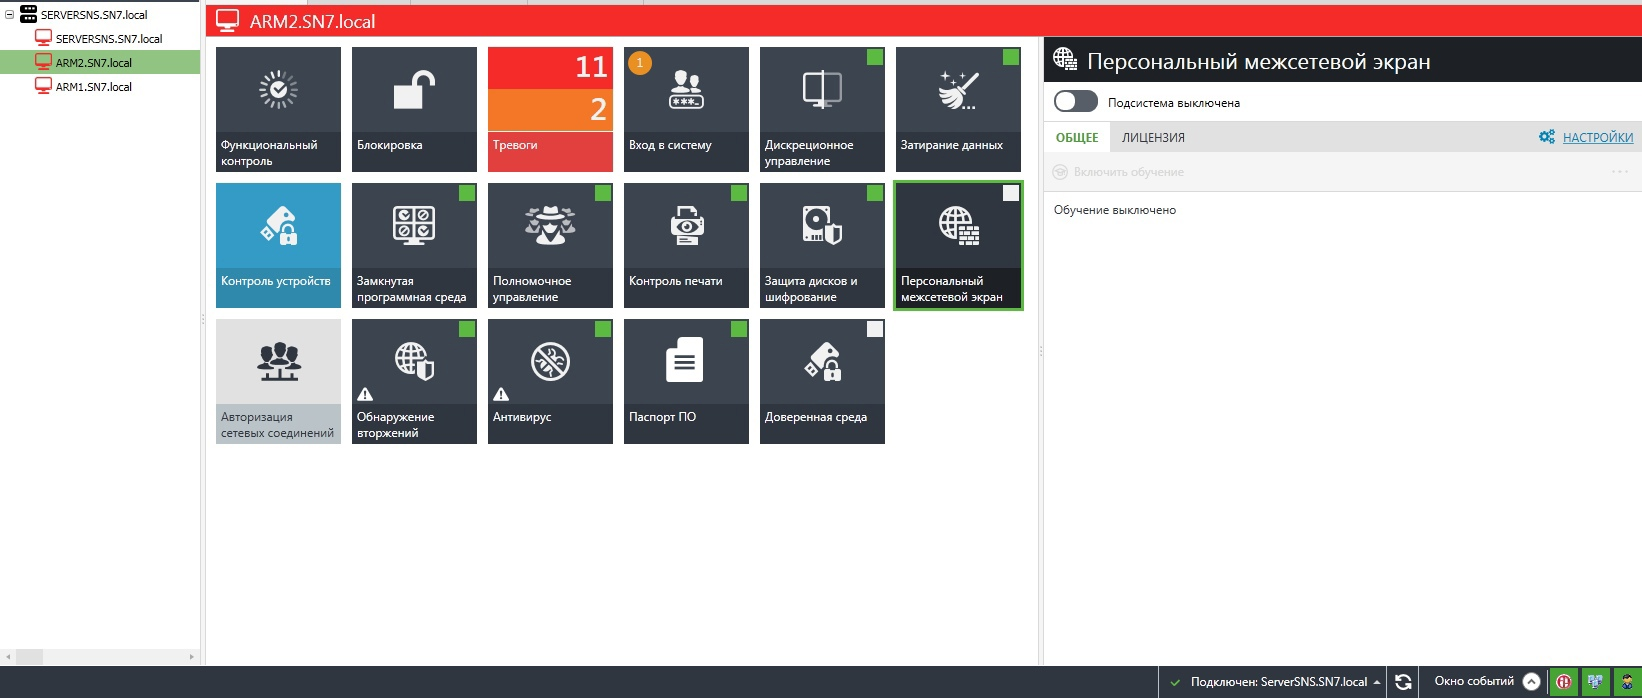
\includegraphics[scale=0.3]{pics/1.jpg}

      Рис 1. Персональный межсетевой экран.
    \end{center}

    \textbf{Пункт 3}
    \vspace{-3ex}
    \begin{center}
        \singlespacing
        В данном пункте мы настроили политики СОВ на клиенте SNS, установленном на СБ.

        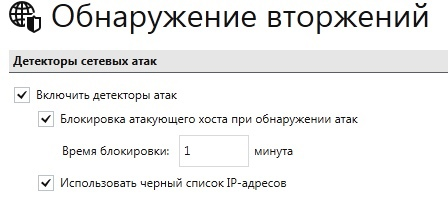
\includegraphics[scale=0.8]{pics/3_1.jpg}

        Рис 2. Основное окно настройки.

        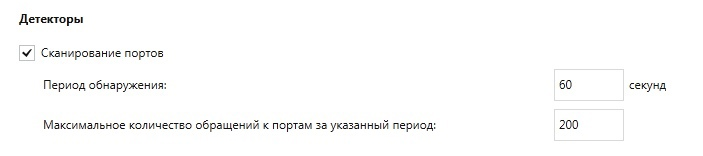
\includegraphics[scale=0.65]{pics/3_2.jpg}

        Рис 3. Детекторы.

        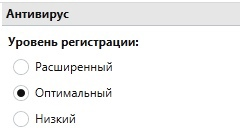
\includegraphics[scale=0.8]{pics/3_3.jpg}
 
        Рис 4. Регистрация событий.
    \end{center}

    \textbf{Пункт 4}
    \vspace{-3ex}
    \begin{center}
        \singlespacing
        В данном пункте мы имитировали атаку на компьютер ServerSNS.

        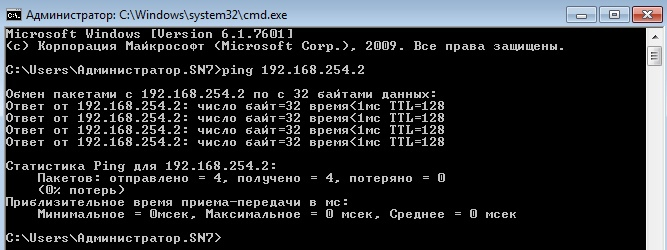
\includegraphics[scale=0.6]{pics/4_1.jpg}
        
        Рис 5. Компьютер ServerSNS доступен.

        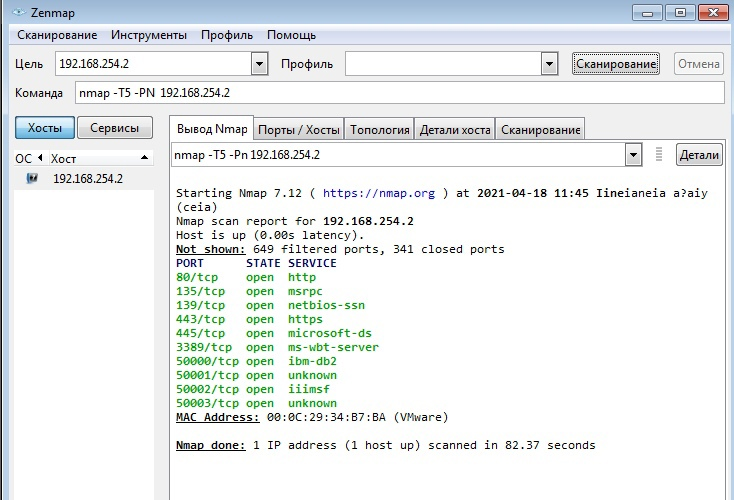
\includegraphics[scale=0.6]{pics/4_2.jpg}

        Рис 6. Проводим сканирование портов защищаемого сервера.

        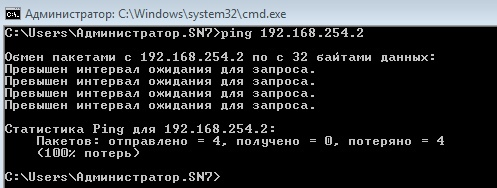
\includegraphics[scale=0.7]{pics/4_3.jpg}

        Рис 7. Компьютер ServerSNS недоступен.

    \end{center}

    \textbf{Пункт 5}
    \vspace{-3ex}
    \begin{center}
        \singlespacing
        В данном пункте мы проверили наличие записи тревоги. 

        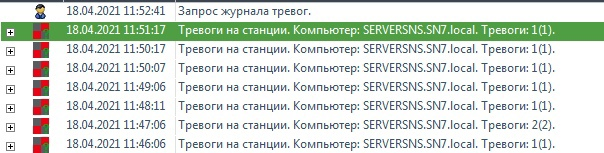
\includegraphics[scale=0.6]{pics/5_1.jpg}

        Рис 8. Появились записи о событиях тревоги на СБ в панели событий.

        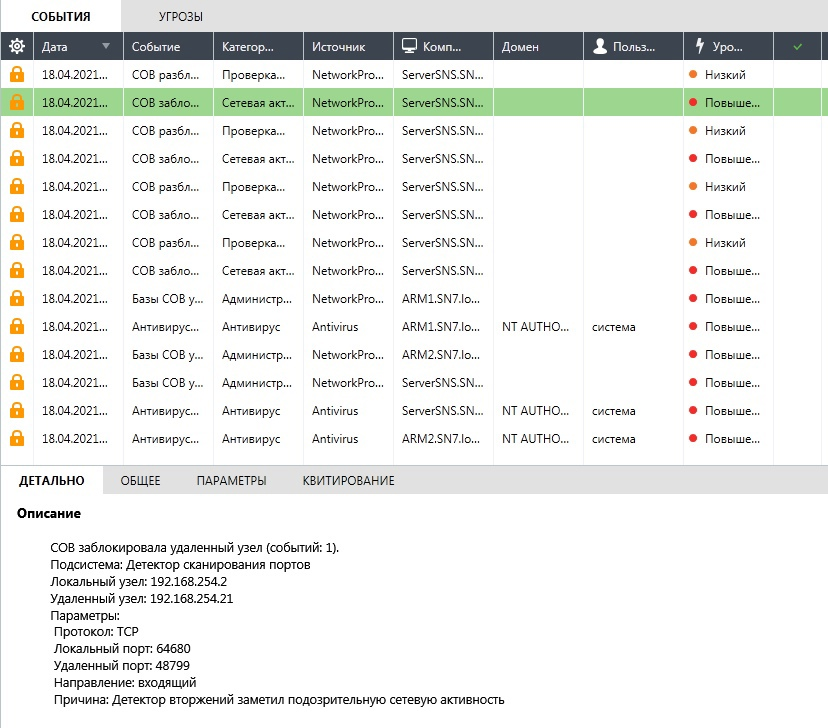
\includegraphics[scale=0.45]{pics/5_2.jpg}

        Рис 9. В журнале тревог появились сообщения о блокировке атакующего узла.

    \end{center}

    \newpage
    \textbf{Пункт 6}
    \vspace{-3ex}
    \begin{center}
        \singlespacing
        В данном пункте мы провели дополнительную настройку политик СОВ на клиенте SNS.

        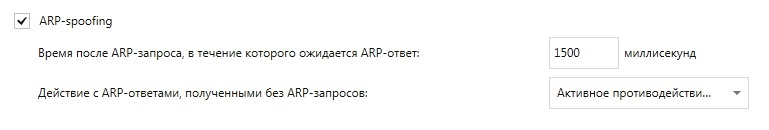
\includegraphics[scale=0.6]{pics/6.jpg}

        Рис 10. ARP-spoofing
    \end{center}

    \textbf{Пункт 7}
    \vspace{-3ex}
    \begin{center}
        \singlespacing
        В данном пункте мы имитировали атаку ARP-spoofing на компьютер ServerSNS.

        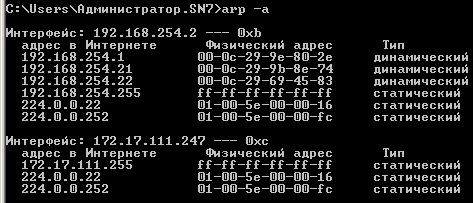
\includegraphics[scale=0.8]{pics/7_1.jpg}
        
        Рис 11. Определяем mac-адрес компьютера.

        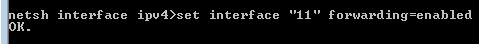
\includegraphics[scale=0.8]{pics/7_2.jpg}

        Рис 12. Переводим интерфейс в статус пересылки ipv4 пакетов.

        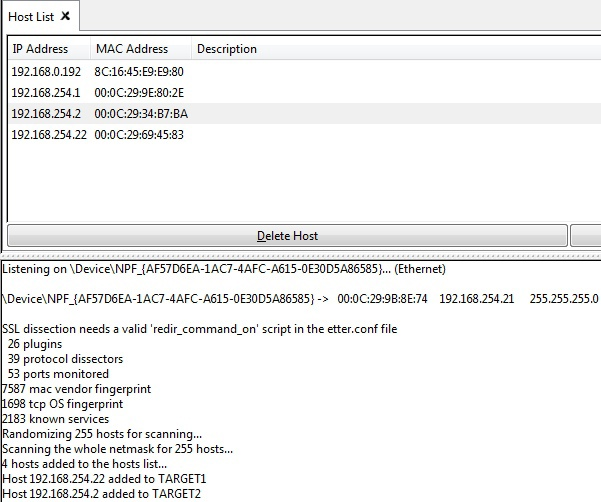
\includegraphics[scale=0.64]{pics/7_3.jpg}

        Рис 13. Список доступных хостов в сети.

        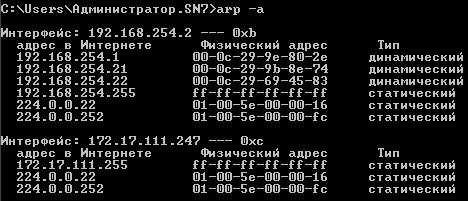
\includegraphics[scale=0.8]{pics/7_4.jpg}

        Рис 14. Убеждаемся, что верно определили mac-адрес.

        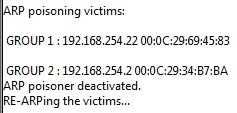
\includegraphics[scale=0.9]{pics/7_5.jpg}

        Рис 15. Останавливаем атаку.
    \end{center}

    \textbf{Пункт 8}
    \vspace{-3ex}
    \begin{center}
        \singlespacing
        В данном пункте мы останавили команду ping.

        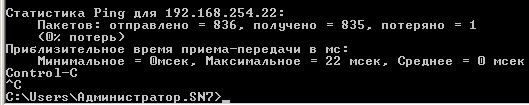
\includegraphics[scale=0.5]{pics/8.jpg}

        Рис 16. Остановка ping
    \end{center}

    \vspace{-2ex}
    \textbf{Пункт 9}
    \vspace{-3ex}
    \begin{center}
        \singlespacing
        В данном пункте мы провели проверку журнала тревог. 

        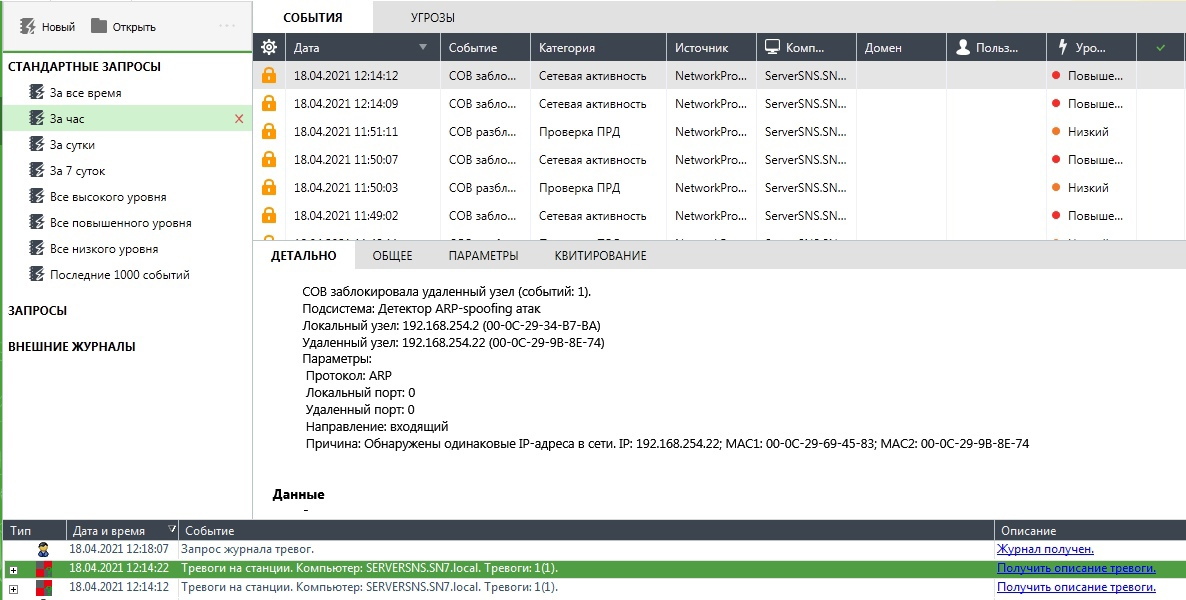
\includegraphics[scale=0.4]{pics/9.jpg}

        Рис 17. В журнале тревог появились сообщения детектора атак об arp-спуфинге
    \end{center}

    \textbf{Вывод}\par
    В ходе данной лабораторной работы была исследована функциональность модулей "Антивирус" и "Система обнаружения вторжений". 
    Также мы протестировали их работоспособность с помощью программ Nmap и Etthercap.

    \textbf{Ответы на контрольные вопросы.}
    \begin{enumerate}
        \singlespacing
        \item \textbf{Какими программными средствами Secret Net Studio выполняется настройка компонентов "Антивирус" и "СОВ"?}\par
        Панель управления SNS, компоненты “Антивирус” и “Обнаружение вторжений”
        \item \textbf{Какие функции защиты реализуются компонентом "Антивирус" в Secret Net Studio?}\par
        Постоянная защита, контекстное сканирование, быстрое/полное сканирование, автопроверка съемных носителей, выбор уровня защиты, выбор объектов для сканирования, список исключений и выбор действий над вирусами.
        \item \textbf{Какие функции защиты реализуются компонентом "СОВ" в Secret Net Studio?}\par
        Детектор сетевых атак, сигнатурный анализ, блокировка доступа к опасным веб-ресурсам.
        \item \textbf{Какое программное средство в Secret Net Studio используется для централизованного обновления антивирусных баз и баз решающих правил на защищаемых компьютерах?}\par
        Сервер обновлений.
    \end{enumerate}

\end{document}

